% $Id: AllegProposal.tex,v 1.8 2000/07/05 21:02:12 culver Exp $
% AllegProposal.tex
% by A. Thall
% 13. Feb 2003
%
% Small edits and a few additions made by R. Roos
% 21 Jan 2007
% Most particularly, the "box" around the thesis statement has been removed,
% section titles have been modified. The section named "Prior work II" has
% been commented out. The \topmargin has been changed to -.5in and the
% change to \parindent has been commented out.
% The filename "nausicaa.eps" has been changed to simply "nausicaa" so that
% pdflatex can be used on the file (and a file named "nausicaa.pdf" has
% been created using the "epstopdf" command).
% Several subsections have been added to illustrate subsection usage.
% The word "comp" has been replaced by "project" or "thesis" throughout.
% Other small changes have been made.
%
% This document provides a sample Senior Project Proposal template for use
% by students in Allegheny's CS and Applied Computing programs.

\NeedsTeXFormat{LaTeX2e}

\documentclass[11pt]{article}
%The following is used by WinEdt to set up cross-referencing to the BibTeX files
%It is NOT commented out---the comment lets it be simply ignored by non-WinEdt LaTeX compilers

%GATHER{mybibtexDB.bib}
\usepackage[utf8]{inputenc}
\usepackage{setspace}
\usepackage{amsmath}
\usepackage{amssymb}
\usepackage{epsfig}
\usepackage{fancybox}
\usepackage{listings}
\usepackage{algo}
\usepackage{url}

\setlength{\textheight}{9in}
\setlength{\textwidth}{6in}
\setlength{\oddsidemargin}{.25in}
\setlength{\topmargin}{-.5in}  % changed from -.25 by RSR on 1/21/07
%\parindent .5in    % commented out by RSR 1/21/07

%put words in the hyphenation statement if you want to enforce
%how LaTeX should break them (or not) at the end of a line.
%\hyphenation{repre-sen-tations problems exact linear}
\hyphenation{itself}

%%%%%
%% Commented out -- RSR, 1/21/07
%%%%%
% The following provides a box to surround the thesis statement
%\newenvironment{Thesis}%
%{\begin{Sbox}\begin{minipage}{.95\linewidth}}%
%{\end{minipage}\end{Sbox}\begin{center}\fbox{\TheSbox}\end{center}}

\title{Relatório Parcial: Ano 1}
\author{Isaac L.\ Santos\ Sacramento \\ Orientador: Mauro Roisenberg}

\begin{document}

% You can specify a language and other options for
% the code-formatting "listings" package
\lstset{language=C++,basicstyle=\small,
        stringstyle=\ttfamily,showstringspaces=false}

\singlespace
\maketitle

\begin{abstract}                % ~350 words max
Este trabalho apresenta como utilizar Lógica Fuzzy para o processamento de imagem. Mais especificamente, 
como detectar arestas em uma imagem. 


são apresentadas as atividades realizadas no primeiro ano de projeto, mais precisamente no
período de março a outubro de 2015. Neste período foram realizados estudos e experimentos relacionados a análise
e quantificação de incerteza na predição de propriedades petrofísicas pós\-inversão. Estas atividades estão descritas
nas seções a seguir.

\end{abstract}

\doublespace
% This sets section-numbering to only include Section and Subsection numbers
\setcounter{secnumdepth}{2}

\section{Introdução}
Detecção de arestas é o nome dado para um conjunto de métodos matemáticos que objetivam a identificação de pontos em uma
imagem digital na qual o brilho da imagem muda rapidamente, ou seja, possui descontinuidade.
Em uma imagem, uma aresta é a curva que segue o caminho de mudança rápida na intensidade da imagem.
Arestas estão sempre associadas com a fronteira entre objetos em uma cena.

A abordagem de lógica fuzzy para processamento de imagens permite o uso de funções de pertinência para definir
o grau para o qual um pixel pertence a uma aresta ou a uma região uniforme. Neste sentido, embora haja
na literatura diferentes algoritmos para detecção de arestas, é possível realizar a mesma tarefa utilizando conjuntos
e regras fuzzy.


\section{Conversão em escala de cinza}

A primeira etapa na aplicação de lógica fuzzy para detecção de arestas em imagens é a conversão de uma imagem RGB para
escala de cinza. A imagem em RGB é representada por um array de 3 dimensões, referentes à intensidade de vermelho, verde e
azul em cada pixel. Com a conversão para escala de cinza, é possível operar sobre um array de apenas duas dimensões.

\section{Cálculo do Gradiente da Imagem}
Os valores da matriz em escala de cinza estão no intervalo $[0 2^8 - 1]$, assim, é necessário escalar a matriz para que seus valores
permaneçam no intervalo $[0 1]$, double-precision.

Para localizar a existência de quebras em regiões uniformes é necessário operar sobre o gradiente da imagem, o qual
deve ser calculado em relação aos eixos x e y. Os gradintes são obtidos por meio da convolução entre a
matriz de double-precision escalonada e um filtro de gradiente. Para efeito deste trabalho, os vetores de filtro de gradiente
utilizados são $G_x  = [-1 1]$ e $G_y = G_x '$, onde $G_y$ é o vetor $G_x$ transposto. As figuras , a seguir exibem as imagens
gradiente de uma das imagens de teste.



\begin{figure}[!ht]
\centering
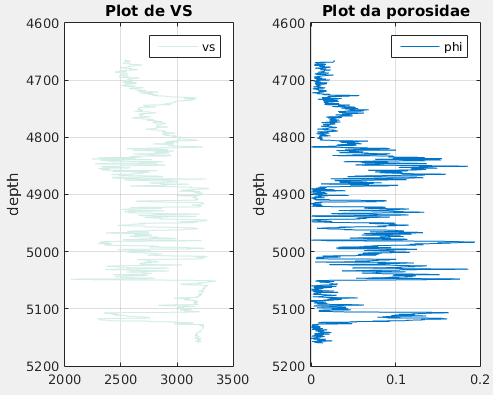
\includegraphics[width=3.0in]{plotvsphi}
\caption{Plot da velocidade cisalhante (Vs) e porosidade (phi).}
\label{fig_grad}
\end{figure}

\section{Definição do Sistema de Inferência Fuzzy}

Neste ponto é necessário criar um Sistema de Inferência Fuzzy (SIF) para modelar as entradas e saídas do sistema desejado.
A plataforma utilizada para o trabalho, MATLAB, possui funções específicas para a criação do sistema de inferência. O sistema
utiliza os gradientes de imagem (nos eixos $x$ e $y$) como entradas.

Os atributos do sistema de inferência criado são parametrizáveis, de modo que o usuário pode ajustar para obter melhores resultados
de acordo com o domínio da aplicação. Considerando que a saída do sistema fuzzy será composta apenas de dois valores (preto e branco)
seguindo as regras fuzzy estabelecidas, foi possível definir como função de pertinência a função gaussiana.

\begin{figure}[!ht]
\centering
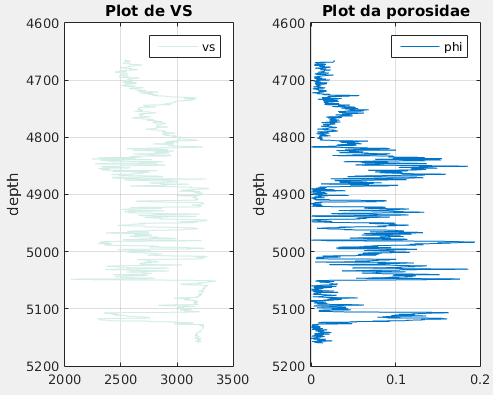
\includegraphics[width=3.0in]{plotvsphi}
\caption{Plot da velocidade cisalhante (Vs) e porosidade (phi).}
\label{fig_plot}
\end{figure}


O terceiro script foi desenvolvido para dar suporte ao módulo de criação dos comitês.
Ele é responsável pela preparação dos dados utilizados no treinamento e teste das redes neurais.
A função recebe como entradas os poços cujos dados serão utilizados para treinar as redes, o poço de teste e as propriedades que se deseja estudar.
Na saída, a função retorna a matriz de dados para treinamento da rede, o vetor do atributo estudado, o vetor de dados de teste  e o vetor de dados
esperados como respostas das redes.

\section{Conclusões}

Os estudos relacionados à análise de incerteza na inversão sísmica com base no método de amostragem por grades esparsas \cite{Tompkins2013} \cite{Tompkins15},
foram suspensos. A análise dos resultados apresentados pelo autores para aplicações em sísmica AVO mostra que o método geométrico, em conjunto
com a inversão convolucional, é mais custoso que a amostragem aleatória em conjunto com o mesmo processo de inversão. Além disso,
a abordagem com grades esparsas, mesmo adicionado o passo de regularização \cite{Tompkins15}, gerou um alto percentual de amostras rejeitadas (mais de 24\%).

A ferramenta de análise de incerteza por comitês de rede neurais, já em forma de protótipo, está em fase de testes e incorporação 
à, já madura, ferramenta de geração de pseudo\-poços. Em conjunto, estas ferramentas devem permitir
ao usuário analisar estatisticamente e utilizar os dados de poços existentes, além de analisar a incerteza dos \textit{logs} dos poços reais e dos pseudo-poços gerados.

 \nocite{*}

\begin{spacing}{1}
   \bibliographystyle{plain}
   \bibliography{mybibtexDB}
 \end{spacing}

\end{document}
